\documentclass[11pt,a4paper]{article}
\usepackage[T1]{fontenc}
\usepackage[utf8]{inputenc}
\usepackage{lmodern}
\usepackage[a4paper,margin=1in]{geometry}
\usepackage{microtype}
\usepackage{xcolor}
\usepackage{hyperref}
\usepackage{booktabs}
\usepackage{tabularx}
\usepackage{longtable}
\usepackage{array}
\usepackage{enumitem}
\usepackage{amsmath}
\usepackage{graphicx}
\usepackage{float}
\usepackage{fancyhdr}
\usepackage{titlesec}
\usepackage{listings}
\usepackage[most]{tcolorbox}
\usepackage[authoryear]{natbib}
\hypersetup{colorlinks=true,linkcolor=blue!50!black,citecolor=blue!50!black,urlcolor=blue!50!black,pdftitle={LDSFL-Meander User Manual},pdfauthor={Lopez-Dubon, Sgarabotto, Frascati and Lanzoni}}

\definecolor{brandblue}{HTML}{1F4E79}
\definecolor{brandteal}{HTML}{2F7C7D}
\definecolor{brandgray}{HTML}{4A4A4A}
\definecolor{boxbg}{HTML}{F4F7FA}

\titleformat{\section}{\large\bfseries\color{brandblue}}{\thesection}{0.6em}{}
\titleformat{\subsection}{\normalsize\bfseries\color{brandteal}}{\thesubsection}{0.6em}{}

\lstdefinestyle{codeblock}{
  basicstyle=\ttfamily\small,
  frame=single,
  backgroundcolor=\color{boxbg},
  columns=fullflexible,
  keepspaces=true,
  breaklines=true,
  showstringspaces=false
}

\newtcolorbox{infobox}[1][]{enhanced,colback=boxbg,colframe=brandblue!55,boxrule=0.6pt,arc=2pt,left=8pt,right=8pt,top=8pt,bottom=8pt,#1}
\newtcolorbox{warnbox}[1][]{enhanced,colback=orange!6,colframe=orange!65!black,boxrule=0.6pt,arc=2pt,left=8pt,right=8pt,top=8pt,bottom=8pt,#1}

\pagestyle{fancy}
\fancyhf{}
\fancyhead[L]{LDSFL-Meander User Manual}
\fancyhead[R]{Lopez-Dubon, Sgarabotto, Frascati and Lanzoni}
\fancyfoot[C]{\thepage}
\setlength{\headheight}{14pt}

\begin{document}

\begin{titlepage}
\centering
\vspace*{1.7cm}
{\Huge\bfseries\color{brandblue}LDSFL-Meander\\[0.4em]}
{\Large A Python Code for a Reduced Two-Dimensional Morphodynamic Model for Meandering Rivers\\[0.8em]}
{\Large User Manual\\[1.2em]}
{\large Sergio Lopez-Dubon$^{*}$, Alessandro Sgarabotto, Alessandro Frascati and Stefano Lanzoni$^{\dagger}$\\[1.0em]}
\texttt{$^{*}$\href{mailto:Sergio.LDubon@ed.ac.uk}{Sergio.LDubon@ed.ac.uk}}\\
\texttt{$^{\dagger}$\href{mailto:stefano.lanzoni@unipd.it}{stefano.lanzoni@unipd.it}}
\vfill
\begin{tcolorbox}[width=0.92\textwidth,colback=boxbg,colframe=brandblue!55,arc=2pt]
\centering
\textbf{What this manual covers}\par\medskip
Installation, repository structure, command-line and GUI workflows, notation policy, dimensional and dimensionless inputs, geometry preprocessing, runtime controls, saved outputs, troubleshooting, and optional executable packaging for the current LDSFL-Meander source package.
\end{tcolorbox}
\vfill
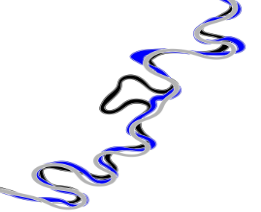
\includegraphics[width=0.42\textwidth]{figures/cover.png}\\[1.2em]
{\large Updated manual for LDSFL-Meander version 0.6.5\\[0.4em]}
{\normalsize \today}
\end{titlepage}

\tableofcontents
\newpage

%%%%%%%%%%%%%%%%%%%%%%%%
\section{Introduction}
\label{Introduction}
%%%%%%%%%%%%%%%%%%%%%%%%

\textbf{LDSFL-Meander} is named after \textbf{Lopez-Dubon, Sgarabotto, Frascati and Lanzoni}. It is a reduced, physics-based, meander-morphodynamics model implemented in Python, with both a command-line runner and a desktop GUI. The theoretical background is described in \citet{FrascatiLanzoni2009}. For more recent developments, not included in this  reduced public release, see \citet{FrascatiLanzoni2013}, \citet{Bogoni2017}, and \citet{LopezDubonLanzoni2019}.

\vspace{0.5em}

 \noindent  LDSFL-Meander is intended for efficient reduced-model studies of channel planform evolution. It is most appropriate for wide, mildly curved, long bends and for reproducible workflow-oriented studies where the user needs to configure cases, run simulations, and inspect planform outputs. It is not intended to replace a fully-fledged 2D or 3D hydrodynamic solver, and fails to address the behaviour of sharp bends.

%%%%%%%%%%%%%%%%%%%%%%%%
\begin{infobox}
\textbf{Core idea.} The solver operates internally in terms of dimensionless quantities. The GUI can accept either dimensionless inputs directly or dimensional hydraulic/sediment inputs that are then converted into the proper internal set of dimensionless parameter before writing the solver input files.
\end{infobox}

%%%%%%%%%%%%%%%%%%%%%%%%
\section{Notation policy and terminology}
\label{Notations}
%%%%%%%%%%%%%%%%%%%%%%%%

Since the project is expected to grow toward more advanced versions, this manual distinguishes between \emph{reference input variables } concerning the initial planform configuration,  (hereafter denoted by a $0$ subscript), and \emph{flow field variables}.

\begin{infobox}
	\textbf{Notation policy used in this manual}
	\begin{itemize}[leftmargin=1.2em]
		\item Software and GUI notation uses user-oriented names and reference quantities. For example, the GUI input reference depth is denoted as $D_0$
		\item The theoretical notation uses intrinsic coordinates $(s,n,z)$ and flow field variables such as $U(s,n)$, $V(s,n)$, $h(s,n)$, and $D(s,n)$.
		\item To avoid ambiguity, this manual indicate the curvature distribution along the channel axis as $\kappa(s)$.
		\item In this manual, $B_0$ denotes the \textbf{reference channel half-width}. The full width is therefore $2B_0$.
	\end{itemize}
\end{infobox}

The complete list of symbols is reported in Section  \ref{SymbolList}.

%%%%%%%%%%%%%%%%%%%%%%%%
\section{Repository overview}
\label{RepositoryOverview}
%%%%%%%%%%%%%%%%%%%%%%%%

\begin{longtable}{>{\small\ttfamily}p{0.38\textwidth} p{0.52\textwidth}}

%\begin{longtable}{p{0.34\textwidth} p{0.56\textwidth}}
\toprule
\textbf{Path} & \textbf{Purpose} \\
\midrule
\endhead
	\texttt{ldsfl/} & Main Python package containing the solver, input handling, GUI utilities, outputs, flow-field routines, resistance closures, and geometry processing \\
	\texttt{run\_ldsfl.py} & Main command-line entry point. Use this when the input CSV files are already prepared \\
	\texttt{gui\_ldsfl.py} & Desktop GUI for setting up and running cases without editing the CSVs manually \\
	\texttt{Run.py} & Convenience local runner for quick local execution \\
	\texttt{Reg.py} & Short regression/smoke runner \\
	\texttt{Input/Parameter.csv} & Case table containing the dimensionless solver inputs \\
	\texttt{Input/xy.csv} & Input file for the channel axis initial geometry \\
	\texttt{smoke\_test.py} & Basic solver smoke test \\
	\texttt{gui\_smoke\_test.py} & GUI/configuration/conversion smoke test \\
	\texttt{README.md} & Project overview.\\
	\texttt{USER\_MANUAL.md} & Short Markdown guide \\
	\texttt{docs/LDSFL\_Meander\_user\_manual.tex} & Full LaTeX user manual source \\
	\texttt{docs/LDSFL\_Meander\_user\_manual.pdf} & Compiled PDF user manual \\
	\texttt{BUILD\_EXE.md} & Notes for building an optional packaged GUI executable \\
	\texttt{CITATION.cff} & Citation metadata for the software release \\
\bottomrule
\label{RepositoryTable}
\end{longtable}

%%%%%%%%%%%%%%%%%%%%%%%%
\section{Installation and first check}
\label{Installation}
%%%%%%%%%%%%%%%%%%%%%%%%

Install the dependencies from the repository root:
\vspace{0.5em}

\begin{lstlisting}[style=codeblock]
	pip install -r requirements.txt
\end{lstlisting}

Then verify the source package:
\vspace{0.5em}

\begin{lstlisting}[style=codeblock]
	python smoke_test.py
	python gui_smoke_test.py
\end{lstlisting}

These tests confirm that the solver runs a short case and that the GUI conversion and configuration path works as expected.

%%%%%%%%%%%%%%%%%%%%%%%%
\section{Quick start}
\label{QuickStart}
%%%%%%%%%%%%%%%%%%%%%%%%

%%%%%%%%%%%%%%%%%%%%%%%%
\subsection{Command line}
\label{CommandLine}
%%%%%%%%%%%%%%%%%%%%%%%%

Use the command line (CLI) when the input files are already prepared:
\vspace{0.5em}

\begin{lstlisting}[style=codeblock]
	python run_ldsfl.py --base-dir . --cases 1 --max-steps 50 --no-plots
\end{lstlisting}

\vspace{0.5em}
The CLI also supports advanced options such as \texttt{--max-sim-time}, \texttt{--stop-mode}, \texttt{--cstab}, geometry filtering controls, and \texttt{--output-units}.

%%%%%%%%%%%%%%%%%%%%%%%%
\subsection{GUI}
\label{GUI}
%%%%%%%%%%%%%%%%%%%%%%%%

Launch the GUI with:
\vspace{0.5em}

\begin{lstlisting}[style=codeblock]
	python gui_ldsfl.py
\end{lstlisting}

\vspace{0.5em}
The GUI is the easiest way to:
\begin{itemize}[leftmargin=1.2em]
	\item choose between dimensionless and dimensional inputs,
	\item validate the channel axis file,
	\item scale and filter geometry before writing \texttt{Input/xy.csv},
	\item choose stop criteria and solver backends,
	\item save and load investigated configurations,
	\item inspect dimensionless converted parameters before the run,
	\item monitor live snapshots and review the final planform overlay.
\end{itemize}

An \textbf{investigated configuration} means one row in \texttt{Input/Parameter.csv}, i.e. one simulation setup with a single set of input parameters.

%%%%%%%%%%%%%%%%%%%%%%%%
%	Figure Example of Main GUI view at startup
%%%%%%%%%%%%%%%%%%%%%%%%
\begin{figure}[H]
	\centering
	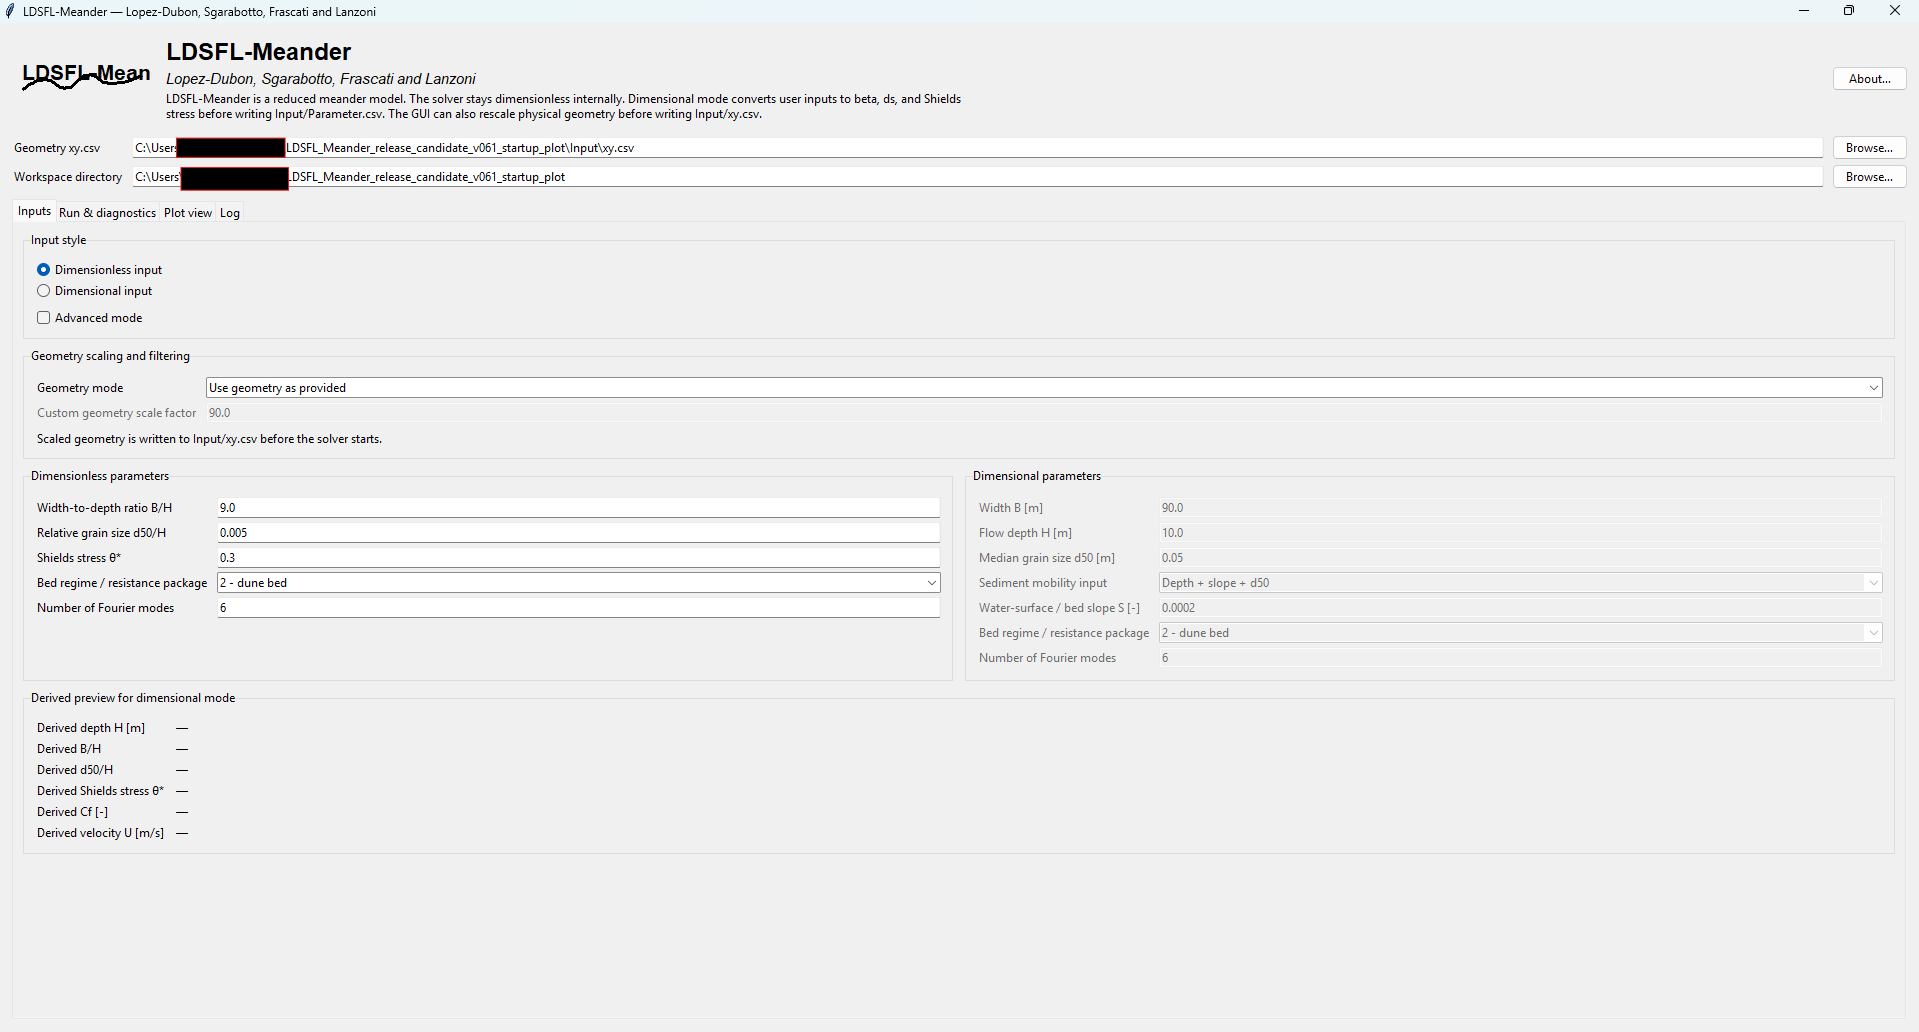
\includegraphics[width=0.97\textwidth]{figures/gui_inputs_default.png}
	\caption{Main GUI view at startup. The interface preloads a bundled example of planform geometry and parameter set (\textit{case study}), such that a first test run can be launched immediately.}
	\label{fig:gui-startup}
\end{figure}

At startup, the GUI loads a default example  (\textit{case study}) of initial planform configuration and input data from the repository. The planform geometry, workspace, and first-row configuration values are already defined, and the example can be run after a quick validation check.

%%%%%%%%%%%%%%%%%%%%%%%%
\section{Input files}
\label{InputFiles}
%%%%%%%%%%%%%%%%%%%%%%%%

%%%%%%%%%%%%%%%%%%%%%%%%
\subsection{Parameter table: \texttt{Input/Parameter.csv}}
%%%%%%%%%%%%%%%%%%%%%%%%

The code reads one row per case study. The corresponding columns are shown below.

%%%%%%%%%%%%%%%%%%%%%%%%
%	Dimensionless input Table
%%%%%%%%%%%%%%%%%%%%%%%%
\begin{table}[H]
	\centering
	\begin{tabularx}{\textwidth}{>{\ttfamily}l >{\raggedright\arraybackslash}X >{\centering\arraybackslash}p{0.15\textwidth}}
	\toprule
	\textbf{Column} & \textbf{Meaning} & \textbf{Units} \\
	\midrule
	Id & Case study identifier used to select the pertinent row & - \\
	Beta & Aspect ratio ($B/D_0$, with $B$ the channel half-width) & - \\
	ds & Relative grain size ($d_{50}/D_0$) & - \\
	Theta & Shields stress, written with the historical CSV spelling used by the code & - \\
	flagbed & Bed-configuration flag. In the current solver: 1 = plane bed, 2 = dune covered bed & - \\
	r & Coefficient accounting fro transverse bed-slope effects on bedload & - \\
	Mdat & Number of Fourier modes retained in the reduced solution & - \\
	\bottomrule
	\end{tabularx}
	\label{TableParameters}
\end{table}

\begin{infobox}
	\textbf{Important notation note.} In this manual, $B_0$ is the channel \textbf{reference half-width}, consistent with the underlying theory. The symbol \texttt{Thetha} (or \texttt{Theta} in some code paths) is retained in the CSV file to denote the dimensionless reference Shields stress, which is written in this manual as $\theta_0$.
\end{infobox}

%%%%%%%%%%%%%%%%%%%%%%%%
\subsection{Geometry file: \texttt{Input/xy.csv}}
%%%%%%%%%%%%%%%%%%%%%%%%

The geometry file stores the initial channel axis coordinates $x$ and $y$ as two columns. The GUI parser accepts:

\begin{itemize}[leftmargin=1.2em]
	\item a first-row header such as \texttt{x,y},
	\item blank lines,
	\item comment lines beginning with \texttt{\#},
	\item extra columns, in which case only the first two are used.
\end{itemize}

Malformed rows, rows with fewer than two columns, or nonnumeric entries are reported with line numbers.

%%%%%%%%%%%%%%%%%%%%%%%%
\section{Dimensionless and dimensional inputs}
\label{Dimensionless and dimensional inputs}
%%%%%%%%%%%%%%%%%%%%%%%%

%%%%%%%%%%%%%%%%%%%%%%%%
\subsection{Dimensionless mode}
%%%%%%%%%%%%%%%%%%%%%%%%

Dimensionless mode is the preferred option, especially when the parameter space needs to be explored.  The main reduced-model parameters are:

\begin{itemize}[leftmargin=1.2em]
	\item aspect ratio $\beta_0 = B_0/D_0$, with $B_0$ the channel half-width,
	\item relative grain size $d_{s0} = d_{50}/D_0$,
	\item Shields stress $\theta_0$,
	\item flag specifying the bed configuration \texttt{flagbed},
	\item number of Fourier modes $M$ (stored as \texttt{Mdat}),
	\item  coefficient  accounting for transverse bed-slope effects on bedload $r$ (available when advanced mode is activated).
\end{itemize}

%%%%%%%%%%%%%%%%%%%%%%%%
\subsection{Dimensional mode}
%%%%%%%%%%%%%%%%%%%%%%%%

Dimensional mode allows the GUI to derive the dimensionless reduced-model parameters from physical variables. Specifically, it computes the initial values of $\beta_0$, $d_{s0}$, and $\theta_0$ before writing \texttt{Input/Parameter.csv}.

%%%%%%%%%%%%%%%%%%%%%%%%
\subsection{Bed shear stress input methods}
\label{ShearStressInput}
%%%%%%%%%%%%%%%%%%%%%%%%

The GUI supports five input methods for specifying the bed shear stress associated to the initial river configuration:

\begin{enumerate}[leftmargin=1.4em]
	\item specification of Shields stress $\tau_{*0}$
	\item specification of  bed shear stress $\tau_{b0}$ and  $d_{50}$,
	\item specification of reference depth $D_0$,  longitudinal slope $S_0$, and $d_{50}$,
	\item specification of reference depth $D_0$, velocity $U_0$,  friction, and $d_{50}$,
	\item specification of discharge $Q$, half-width $B_0$, longitudinal slope $S_0$, friction, and $d_{50}$.
\end{enumerate}

%%%%%%%%%%%%%%%%%%%%%%%%
\section{Friction options}
\label{FrictionOptions}
%%%%%%%%%%%%%%%%%%%%%%%%

The GUI accepts four friction representations:

\begin{itemize}[leftmargin=1.2em]
	\item friction coefficient $c_{f0}$ (-),
	\item Darcy-Weisbach coefficient $f_0$ (-),
	\item Ch\'ezy coefficient $C_{C0}$ (m$^{1/2}$/s),
\item Manning coefficient $n_{M0}$ (s/m$^{1/3}$).
\end{itemize}

%%%%%%%%%%%%%%%%%%%%%%%%
\subsection{Conversion formulas used by the GUI}
%%%%%%%%%%%%%%%%%%%%%%%%

The GUI uses the following conversion relations, depending on the options reported  in \ref{ShearStressInput} and 
\ref{FrictionOptions}:

\begin{subequations}
\begin{align}
	\beta_0 &= \frac{B_0}{D_0}, \\
	d_{s0} &= \frac{d_{50}}{D_0}, \\
	\theta_0 &= \frac{\tau_{b0}}{(\rho_s - \rho) \,g \, d_{50}}, &&  \text{(method \ref{ShearStressInput}.2)}, \\
	\theta_0 &= \frac{\rho \, D_0 \, S_0 }{(\rho_s - \rho) \, d_{50}}, && \text{(method \ref{ShearStressInput}.3)},\\
	\theta_0 &= \frac{\rho \, c_{f0} \, U_0^2}{(\rho_s - \rho) \,g\,d_{50}}, &&  \text{(method \ref{ShearStressInput}.4)},  \\
	c_{f0} &= \frac{f}{8}, &&  \text{(method \ref{FrictionOptions}.2)}, \\
	c_{f0} &= \frac{g}{C_{C0}^2}, && \text{(method \ref{FrictionOptions}.3)}, \\
	c_{f0} &= \frac{g \, n_{M0}^2}{D_0^{1/3}}, &&\text{(method \ref{FrictionOptions}.4)}, \\
	D_0 &= \left(\frac{Q \, n_{M0}}{2 \, B \sqrt{S_0}}\right)^{3/5}, &&   \text{(method \ref{ShearStressInput}.5 with Manning)}, \\
	D_0 &= \left(\frac{Q}{2 \, B\sqrt{g \, S_0/c_{f0}}}\right)^{2/3}, && \text{(method \ref{ShearStressInput}.5 with friction coefficient)},.
\end{align}
\end{subequations}

For the \ref{ShearStressInput}.5  method, the GUI estimates the reference depth $D_0$ using either the initial Manning or friction coefficient before computing $\theta_0$.

%%%%%%%%%%%%%%%%%%%%%%%%
\section{Geometry preprocessing}
%%%%%%%%%%%%%%%%%%%%%%%%

%%%%%%%%%%%%%%%%%%%%%%%%
\subsection{Geometry scaling modes}
%%%%%%%%%%%%%%%%%%%%%%%%

The GUI can write the imported channel axis geometry in two ways:
\begin{itemize}[leftmargin=1.2em]
	\item use geometry as provided,
	\item scale $x$ and $y$ by the half-width $B_0$.
\end{itemize}

Note that the solver entails the channel axis geometry normalised by the reference channel half-width $B_0$.

%%%%%%%%%%%%%%%%%%%%%%%%
\subsection{Advanced geometry controls}
%%%%%%%%%%%%%%%%%%%%%%%%

Advanced mode includes geometry filtering controls:
\begin{itemize}[leftmargin=1.2em]
	\item \textbf{Enable geometry smoothing/filtering} -- turn the smoothing stage on/off.
	\item \textbf{Geometry smoothing factor} -- controls how strongly short-scale noise is damped.
	\item \textbf{Neck cutoff interval} -- check for neck cutoffs every $N$ iterations. Set this to 0 to disable neck-cutoff checks.
	\item \textbf{Resample upper factor} -- trigger resampling when mean point spacing becomes too large.
	\item \textbf{Resample lower factor} -- trigger resampling when mean point spacing becomes too small.
\end{itemize}

\begin{warnbox}
	These parameters affect curvature estimation and cutoff behavior. Use the default values first, and only tune them when you have specific numerical or scientific reasons.
\end{warnbox}

%%%%%%%%%%%%%%%%%%%%%%%%
% Figure Example of advance input
%%%%%%%%%%%%%%%%%%%%%%%%
\begin{figure}[H]
\centering
	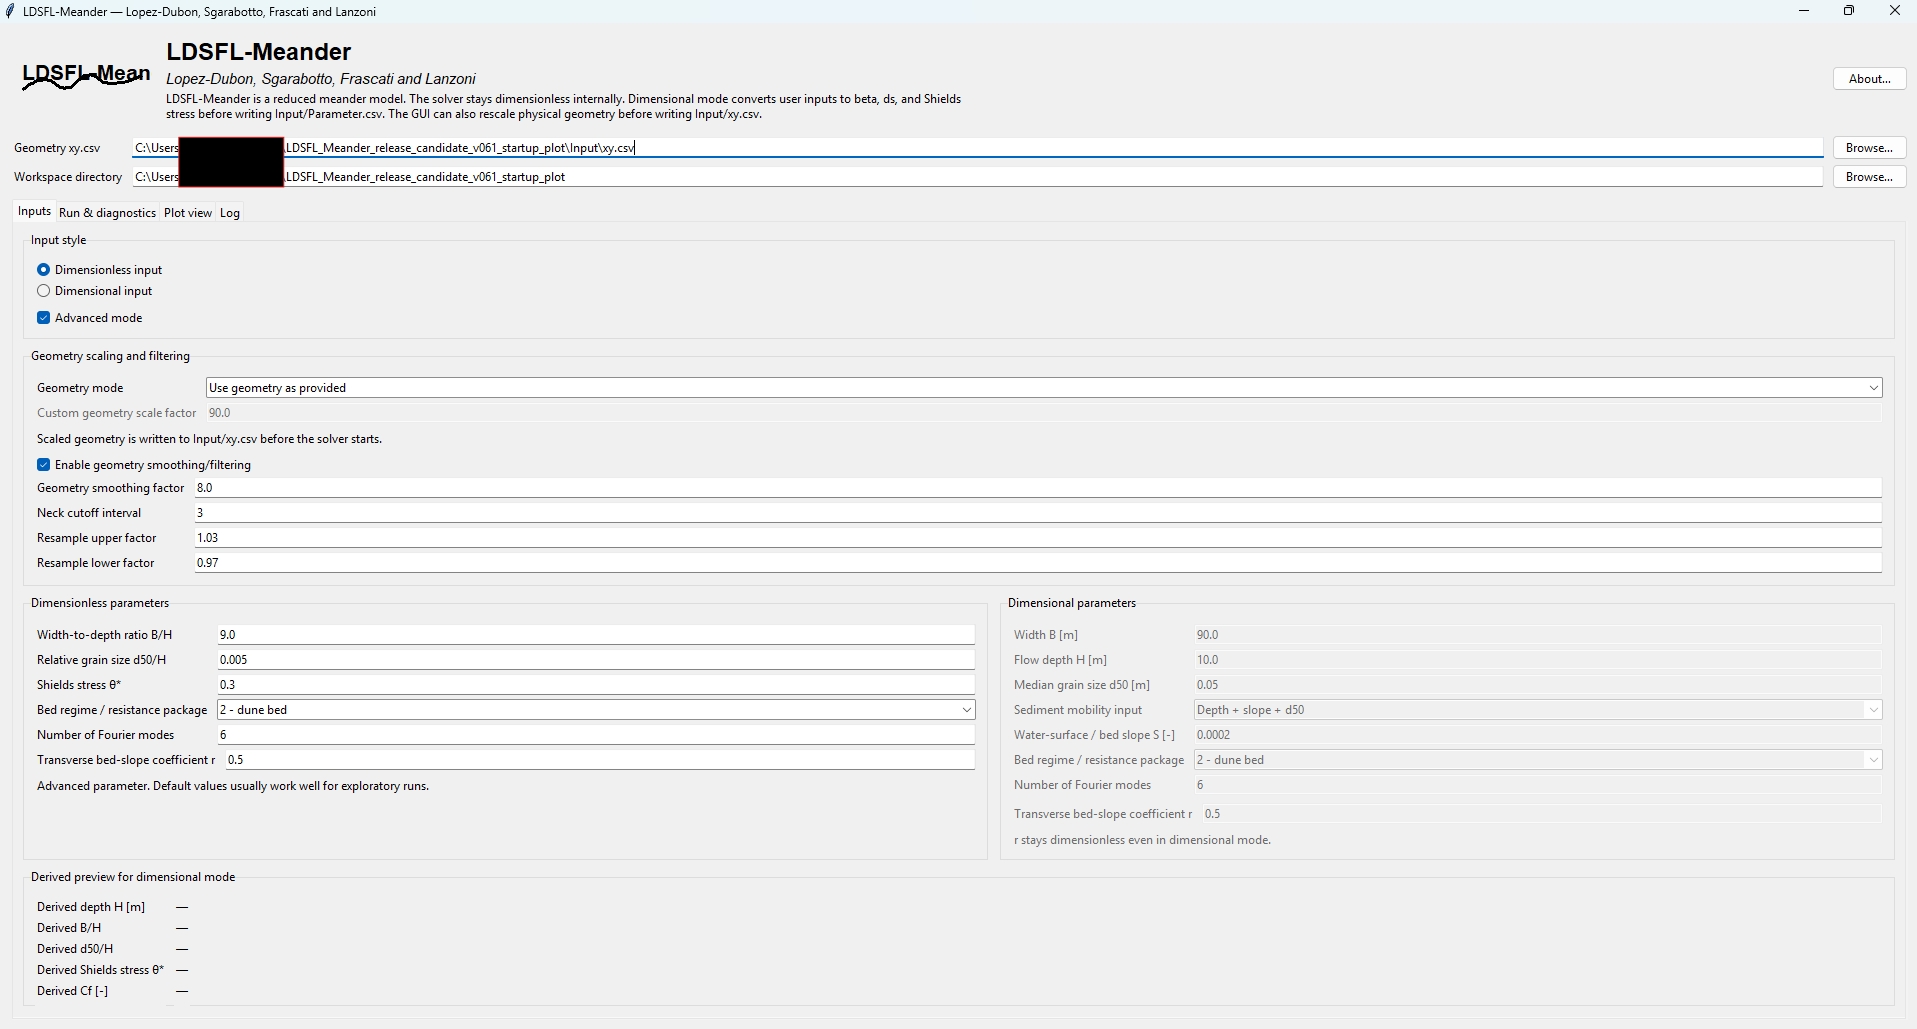
\includegraphics[width=0.97\textwidth]{figures/gui_inputs_advanced.png}
	\caption{Example of advanced input view enabling geometry scaling/filtering controls and changing the parameter $r$ accounting for transverse bed slope effects on bedload. These controls should normally be changed only when thereare clear numerical or scientific reasons.}
	\label{fig:gui-advanced-inputs}
\end{figure}

%%%%%%%%%%%%%%%%%%%%%%%%
\subsection{Why scaling and filtering matter}
%%%%%%%%%%%%%%%%%%%%%%%%

The reduced solver is sensitive to curvature, spacing of channel axis discretization, and geometric noise. In practice, a useful workflow is:

\begin{enumerate}[leftmargin=1.4em]
	\item validate the imported channel axis description,
	\item rescale it if needed,
	\item apply mild smoothing if the source geometry is noisy,
	\item keep the default resampling factors unless you have good reasons to change them.
\end{enumerate}

%%%%%%%%%%%%%%%%%%%%%%%%
\section{Flexible stop criteria}
%%%%%%%%%%%%%%%%%%%%%%%%

Both the GUI and CLI support three criteria for stopping simulations:

\begin{itemize}[leftmargin=1.2em]
	\item \textbf{ steps}: maximum number of steps,
	\item \textbf{time}: maximum simulated time,
	\item \textbf{cutoffs}: maximum number of cutoffs.
\end{itemize}

Each criterion can be enabled or disabled. If only one criterion is enabled, the run behaves as a single-criterion stop.

%%%%%%%%%%%%%%%%%%%%%%%%
\subsection{Combining stopping criteria}
%%%%%%%%%%%%%%%%%%%%%%%%

Two combination rules are available:
\begin{itemize}[leftmargin=1.2em]
	\item \textbf{first} -- stop the simulation as soon as the first enabled criterion is reached,
	\item \textbf{all} -- stop the simulation only when all enabled criteria have been reached.
\end{itemize}

\begin{infobox}
	For most users, the safest setup is \textbf{steps} and \textbf{cutoffs}, leaving \textbf{time} disabled initially, and use \textbf{first} as combination rule.
\end{infobox}

%%%%%%%%%%%%%%%%%%%%%%%%
\section{Advanced solver controls}
%%%%%%%%%%%%%%%%%%%%%%%%

The GUI includes an \textbf{Advanced solver controls} panel.

\subsection{Boundary condition}

Following \cite{LanzoniSeminara2006}, the following boundary conditions can be selected:

\begin{itemize}[leftmargin=1.2em]
	\item \textbf{free} -- open-boundary/free-flow configuration,
	\item \textbf{periodic} -- repeating-domain/periodic-flow configuration.
\end{itemize}

\subsection{Backend}
\begin{itemize}[leftmargin=1.2em]
	\item \textbf{numpy} -- reference implementation,
	\item \textbf{numba} -- JIT-accelerated implementation for supported free-boundary calculations.
\end{itemize}

\subsection{Additional controls}

\begin{itemize}[leftmargin=1.2em]
	\item \textbf{cstab} -- timestep stability coefficient.
	\item \textbf{Parallel flow flag} -- low-level parallel mode switch.
	\item \textbf{Flow workers} -- worker count for the parallel-flow option.
	\item \textbf{Numba parallel} -- enable Numba parallel kernels where supported.
	\item \textbf{Numba fastmath} -- enable  Numba fast-math optimisations.
	\item \textbf{Sinuosity stability window} -- number of stored sinuosity values used to decide whether the planform is stable or quasi-stable. The recommended default is 100.
	\item \textbf{Sinuosity relative tolerance} -- tolerance used for the stability check. The default value 0.005 corresponds to about 0.5\% relative spread.
\end{itemize}

\subsection{Recommended default settings}

\begin{itemize}[leftmargin=1.2em]
	\item start with \textbf{free + numpy},
	\item then try \textbf{free + numba} if Numba is installed and you want faster runs,
	\item keep \textbf{cstab = 0.01} initially,
	\item leave \textbf{Parallel flow flag = 0} unless you are testing that path.
\end{itemize}

%%%%%%%%%%%%%%%%%%%%%%%%
%. Figure  Example of tun and Diagnostic Tab
%%%%%%%%%%%%%%%%%%%%%%%%
\begin{figure}[H]
	\centering
	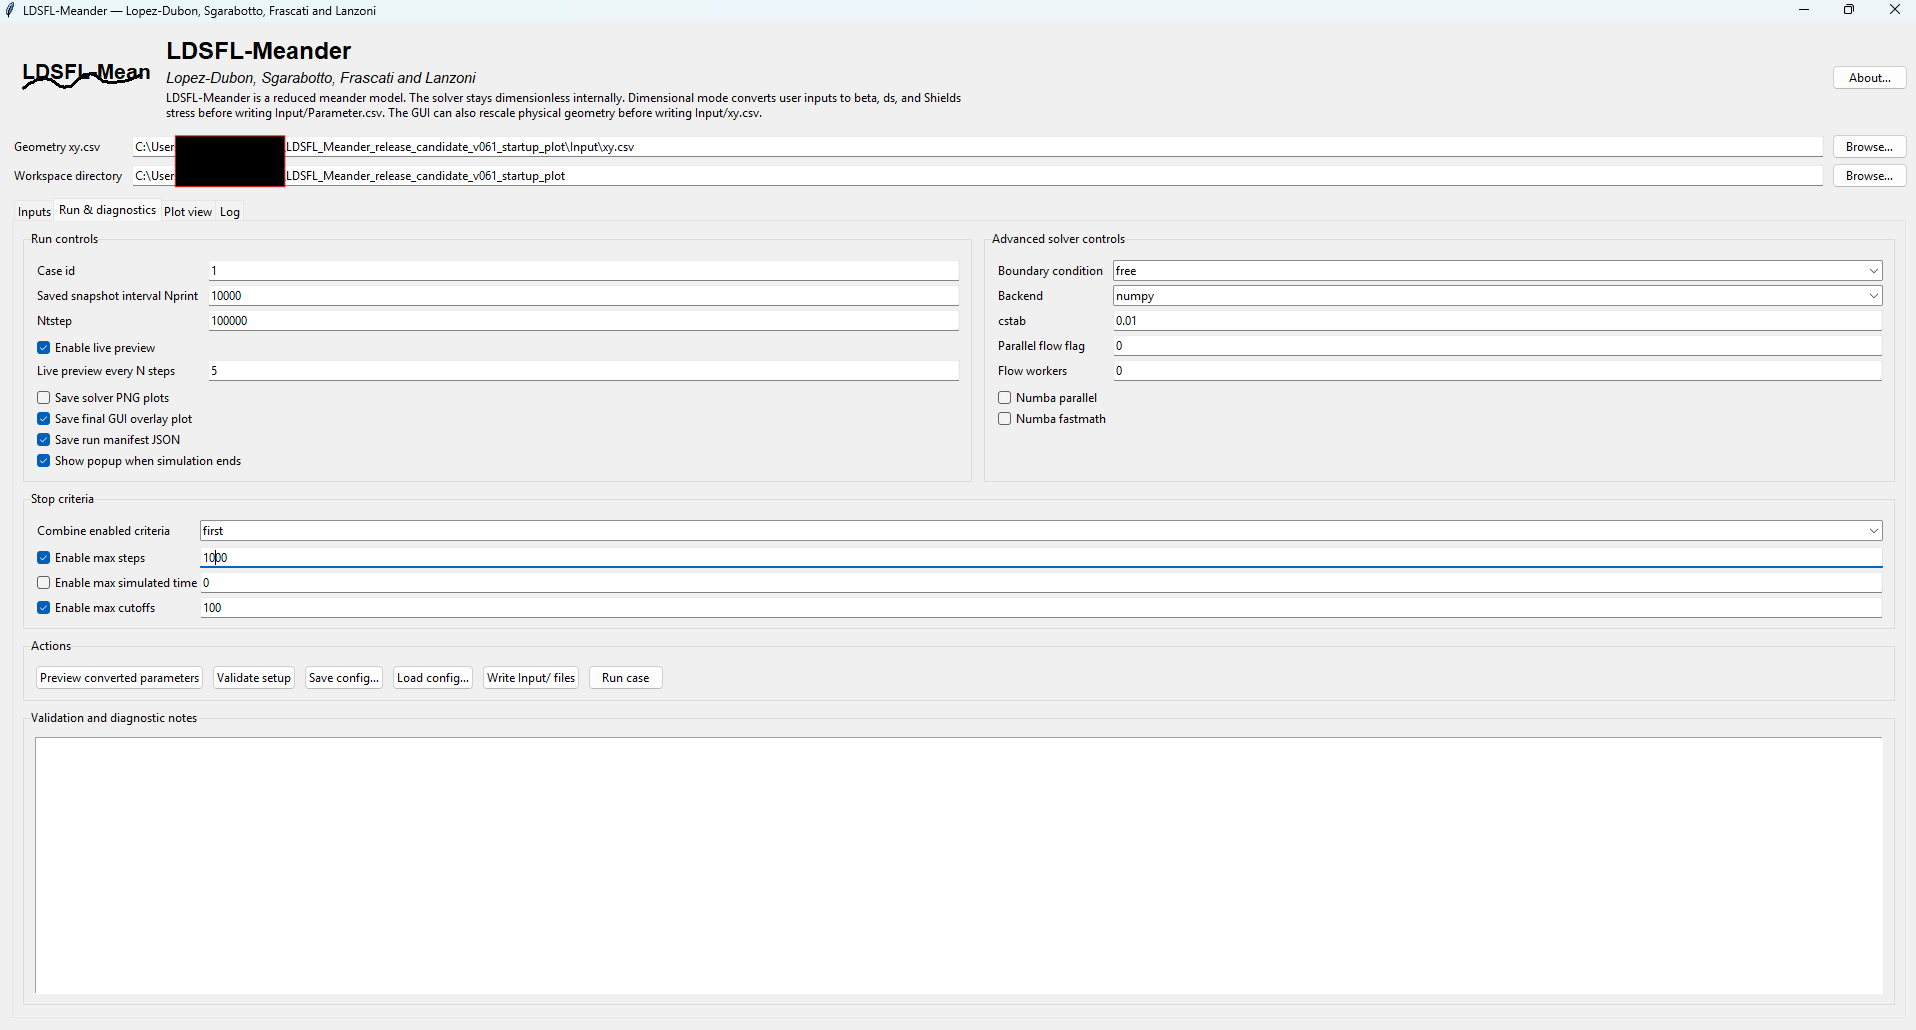
\includegraphics[width=0.97\textwidth]{figures/gui_run_diagnostics.png}
	\caption{Example of run and diagnostics panel, including runtime controls, advanced solver options, output-unit selection, optional saved outputs, flexible stop criteria, and actions such as validation, config save/load, and case study execution.}
	\label{fig:gui-run-diagnostics}
\end{figure}

%%%%%%%%%%%%%%%%%%%%%%%%
\section{Plot view, notifications, and saved outputs}
%%%%%%%%%%%%%%%%%%%%%%%%

The GUI plot tab shows:

\begin{itemize}[leftmargin=1.2em]
	\item the initial channel axis geometry,
	\item the latest live snapshot when available,
	\item the final planform after the simulation finishes.
\end{itemize}

The user can also choose whether the initial channel axis geometry should remain visible on the overlay plot.

\vspace{0.5em}
The plot title is intentionally kept at the top of the panel, while the legend is placed at the upper-left corner of the plotting area such that the curve comparison remains easy to read even for long, low-amplitude planforms.

%%%%%%%%%%%%%%%%%%%%%%%%
% Figure Plot view
%%%%%%%%%%%%%%%%%%%%%%%%
\begin{figure}[H]
	\centering
	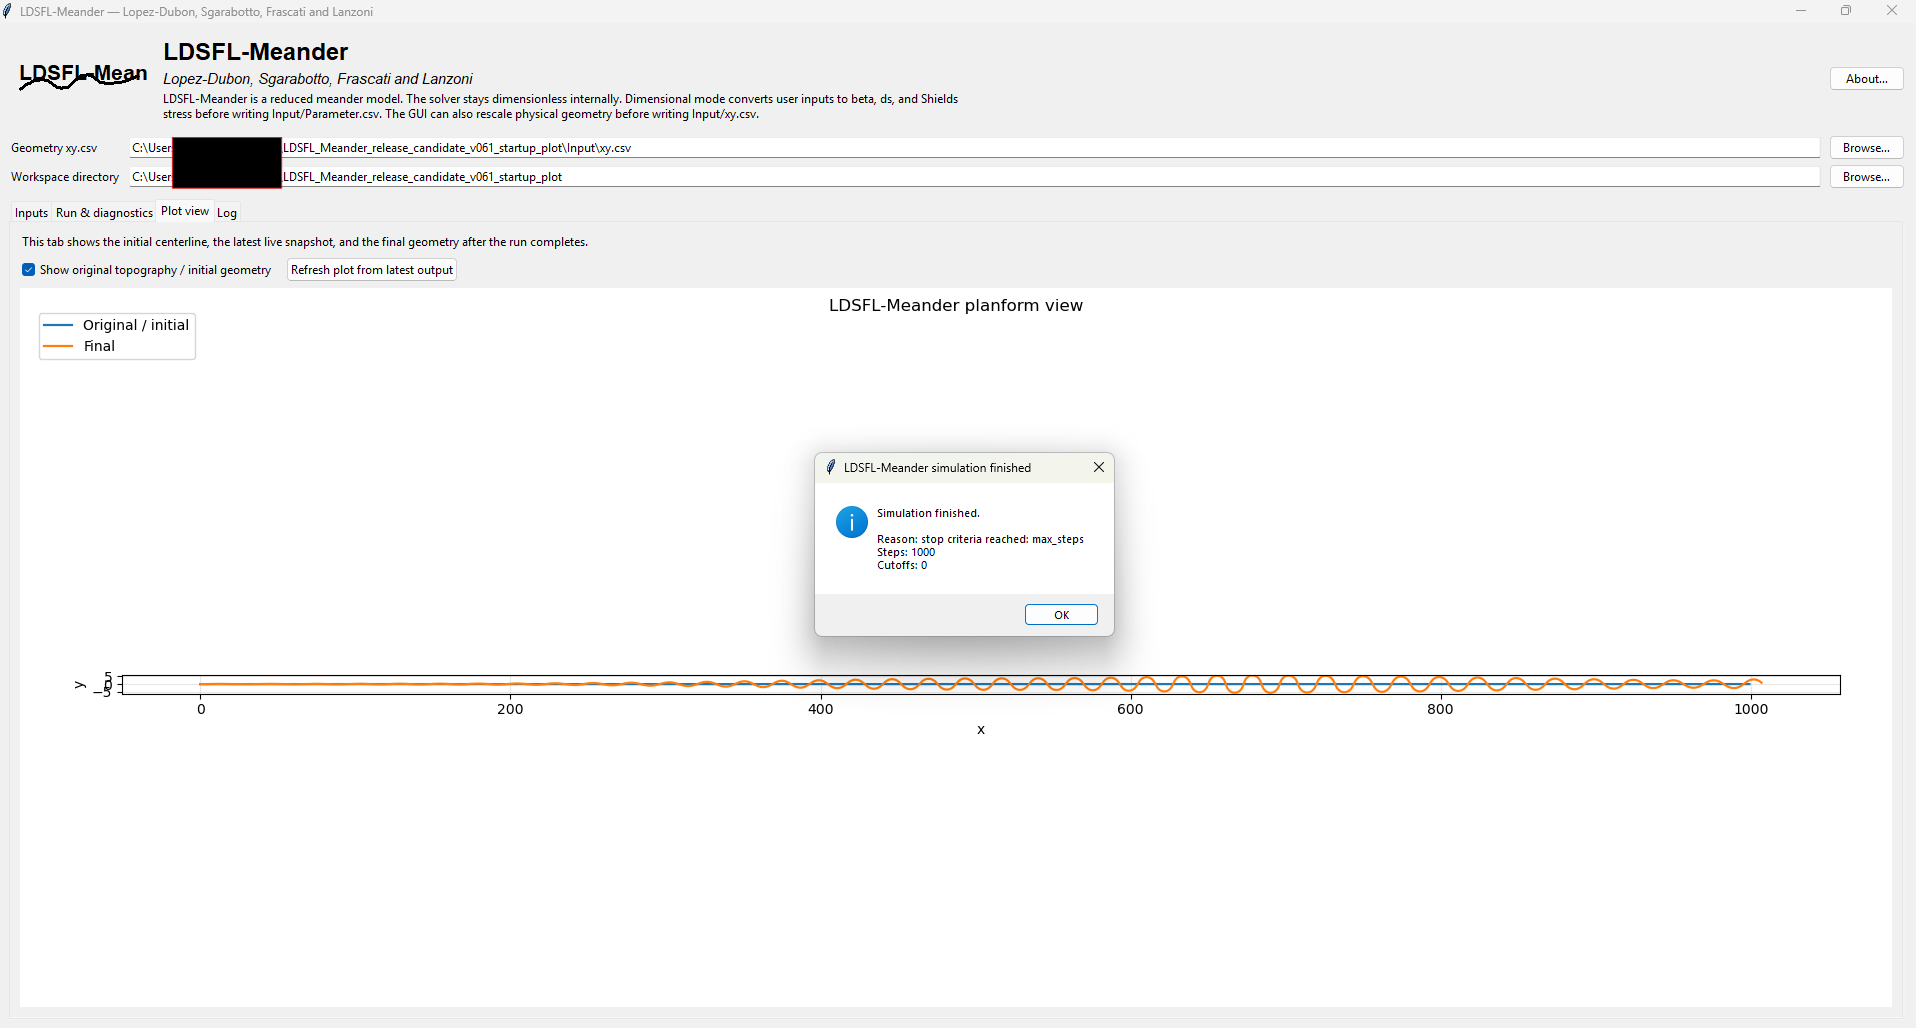
\includegraphics[width=0.97\textwidth]{figures/gui_plot_view.png}
	\caption{Example of plot view at the end of a simulation. The original and final channel centreline are overlaid, the legend is placed at the upper-left of the plotting area, and a completion popup reports the stopping reason and summary values.}
	\label{fig:gui-plot-view}
\end{figure}

%%%%%%%%%%%%%%%%%%%%%%%%
\subsection{Optional saved outputs}
%%%%%%%%%%%%%%%%%%%%%%%%

The GUI can also save:

\begin{itemize}[leftmargin=1.2em]
	\item \texttt{gui\_final\_overlay.png} -- the final GUI overlay plot,
	\item \texttt{run\_manifest.json} -- a machine-readable summary of the resolved inputs and simulation result.
\end{itemize}

The run controls also include an \textbf{Output units} selector:
\begin{itemize}[leftmargin=1.2em]
	\item \textbf{dimensionless} keeps the saved solver outputs in the internal reduced variables used by the code,
	\item \textbf{dimensional} rescales saved coordinates and the saved velocity field back to dimensional form when dimensional input mode is used. Lengths are rescaled with the same geometry scale selected in the GUI (typically $B_0$), while velocity is rescaled with the resolved reference velocity $U_0$.
\end{itemize}
If dimensional outputs are requested while only dimensionless inputs are provided, the code falls back to dimensionless outputs.


\subsection{Scrollable tabs, stop, and continuation}

Version 0.6.5 adds vertical scrollbars to the \textbf{Inputs} and \textbf{Run \& diagnostics} tabs. This keeps the run controls, sinuosity panel, and diagnostic notes accessible on smaller laptop screens.

The \textbf{Run \& diagnostics} tab also includes two controls for long or iterative simulations:
\begin{itemize}[leftmargin=1.2em]
    \item \textbf{Stop after current step} requests a graceful stop. The solver finishes the current safe iteration boundary, writes a final geometry snapshot, and saves the current sinuosity history.
    \item \textbf{Continue from latest output} starts a new solver segment from the latest saved \texttt{xyu} geometry. This is useful if a run stops because a stop criterion was reached but the planform or sinuosity diagnostic is not yet stable.
\end{itemize}

For a continuation run, the GUI writes \texttt{Input/xy\_continue\_from\_latest.csv} from the latest saved centerline and then runs another segment with the same model parameters. If outputs were saved in dimensional units, the GUI converts the latest coordinates back to solver units before continuing.

\subsection{Sinuosity stability diagnostic}

The GUI includes a \textbf{Sinuosity stability} panel. This panel plots the current history of step number versus sinuosity, and reports a qualitative state: \textbf{not stable}, \textbf{quasi-stable}, or \textbf{stable}. The default window uses the last 100 stored sinuosity values. The stability assessment combines two measures: the relative span of sinuosity over the window and the relative trend per step obtained from a straight-line fit. This is intended as a practical convergence diagnostic for identifying when planform sinuosity has become approximately stable.

The solver also saves this diagnostic in the output folder as:
\begin{itemize}[leftmargin=1.2em]
	\item \texttt{files/sinuosity\_history\_<id\_files>.csv},
	\item \texttt{plot/sinuosity\_history\_<id\_files>.png}.
\end{itemize}

%%%%%%%%%%%%%%%%%%%%%%%%
\subsection{Completion popup}
%%%%%%%%%%%%%%%%%%%%%%%%

The GUI can optionally display a popup when a simulation:

\begin{itemize}[leftmargin=1.2em]
	\item finishes successfully,
	\item stops because the stopping criteria were met,
	\item fails with an error.
\end{itemize}

%%%%%%%%%%%%%%%%%%%%%%%%
% Figure Log Tab example
%%%%%%%%%%%%%%%%%%%%%%%%
\begin{figure}[H]
	\centering
	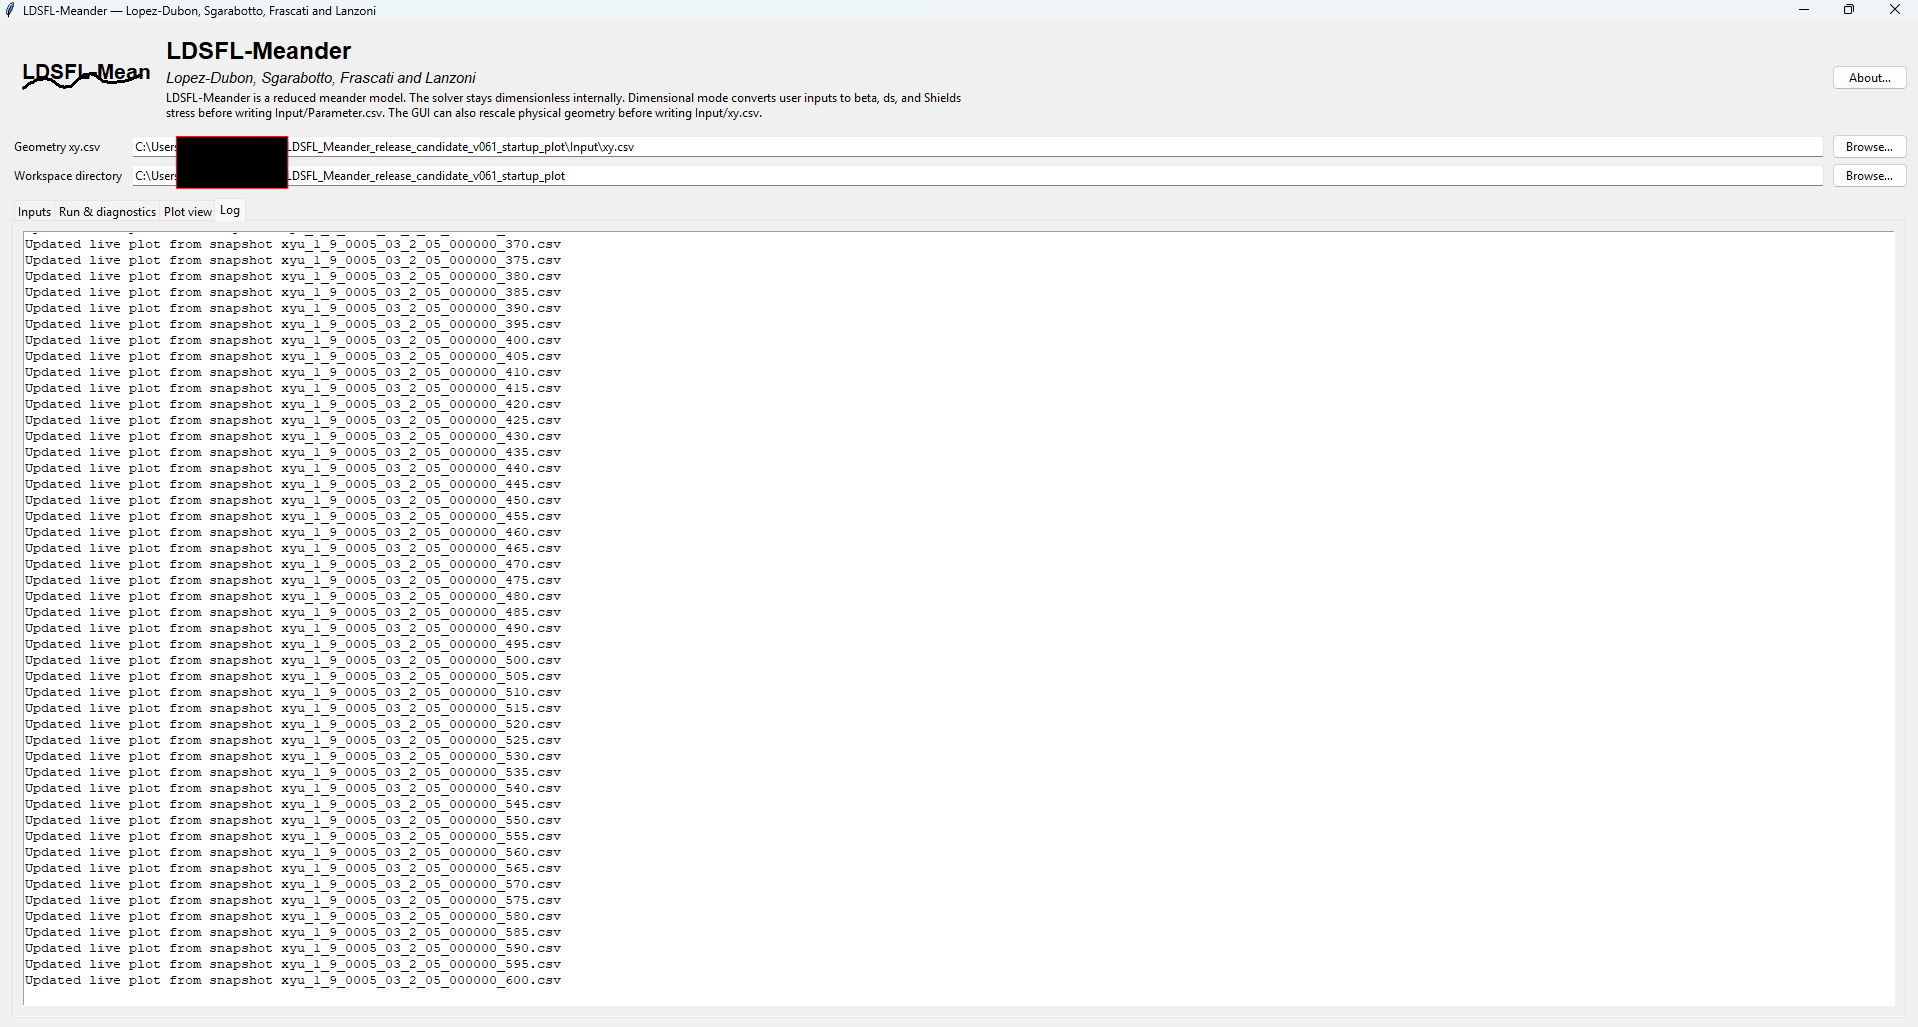
\includegraphics[width=0.97\textwidth]{figures/gui_log.png}
	\caption{Example of Log tab during a simulation. The log tab records snapshot updates, status messages, and diagnostics, and is useful for verifying that live preview and saved outputs are progressing as expected.}
	\label{fig:gui-log}
\end{figure}

%%%%%%%%%%%%%%%%%%%%%%%%
\section{Output folders}
%%%%%%%%%%%%%%%%%%%%%%%%

For each case, LDSFL-Meander creates:

\vspace{0.5em}
\begin{lstlisting}[style=codeblock]
Output/
  <id_files>/
    files/
    plot/
    xy_cut/
    xyu/
\end{lstlisting}

\vspace{0.5em}
Main outputs include:

\begin{itemize}[leftmargin=1.2em]
	\item \texttt{xyu/} -- channel-axis and velocity tables through time,
	\item \texttt{files/} -- tables of saved run variables,
	\item \texttt{plot/} -- planform figures when solver plotting is enabled,
	\item \texttt{xy\_cut/} -- cutoff segments,
	\item \texttt{run\_manifest.json} -- resolved inputs and run summary if enabled,
	\item \texttt{gui\_final\_overlay.png} -- final GUI overlay plot if enabled.
\end{itemize}

%%%%%%%%%%%%%%%%%%%%%%%%
\section{Glossary of variables and controls}
%%%%%%%%%%%%%%%%%%%%%%%%

%%%%%%%%%%%%%%%%%%%%%%%%
\subsection{Reference inputs and reduced parameters}
\label{SymbolList}
%%%%%%%%%%%%%%%%%%%%%%%%

%%%%%%%%%%%%%%%%%%%%%%%%
% Table List of Symbols
%%%%%%%%%%%%%%%%%%%%%%%%
\begin{longtable}{p{0.18\textwidth} p{0.56\textwidth} >{\centering\arraybackslash}p{0.16\textwidth}}
\toprule
\textbf{Symbol / name} & \textbf{Meaning} & \textbf{Units} \\
\midrule
\endhead

% Group 1: Dimensionless inputs
\multicolumn{3}{l}{\textit{Reference flow variables entered by the user in dimensionless mode}} \\
\midrule
$\beta_0$       & Aspect ratio, $B_0/D_0$ & - \\
$d_{s0}$         & Relative grain size, $d_{50}/D_0$ & - \\
$\theta_0$      & Shields stress & - \\
\texttt{flagbed} & Bed-regime flag: 1 = flat bed; 2 = dune covered bed & - \\
$r$           & Coefficient controlling transverse slope effects on bedload & - \\
$M$ / \texttt{Mdat} & Number of Fourier modes retained in the reduced solution & - \\
$cstab$       & Timestep stability coefficient & - \\
\midrule

% Group 2: Dimensional inputs
\multicolumn{3}{l}{\textit{Reference flow variables entered by the user in dimensional mode}} \\
\midrule
$B$           & Channel half-width. The full width is $2B$ & m \\
$D_0$         & Flow depth & m \\
$d_{50}$      & Median sediment grain size & m \\
$S_0$           & Reach-averaged slope & - \\

$Q$           & Water discharge, used in the discharge-based dimensionless conversion method & m$^3$/s \\
$U_0$           & Mean flow velocity, used in the velocity-based dimensionless conversion method & m/s \\
$\tau_{b0}$      & Bed shear stress used in the bed shear stress-based dimensionless conversion  method & Pa = N/m$^2$ \\
$f_0$           & Darcy-Weisbach friction factor, used to compute the friction coefficient as  $c_{f0}=f_0/8$ & - \\
$C_{C0}$         & Ch\'ezy coefficient,  used to compute the friction coefficient as  $c_{f0}=g/C_{C0}^2$. & m$^{1/2}$/s \\
$n_M$ & Manning coefficient;  used to compute the friction coefficient as  $c_f = g \, n_M^2/D_0^{1/3}$ & s/m$^{1/3}$ \\
\midrule

% Group 3: Computed dimensionless quantities
\multicolumn{3}{l}{\textit{Variables computed for generating the dimensionless input table}} \\
\midrule
$c_{f0}$         & Friction coefficient computed from the user-supplied friction parameter and used internally by the solver. & - \\
\bottomrule
\end{longtable}


%%%%%%%%%%%%%%%%%%%%%%%%
\subsection{Geometry and future field notation}
%%%%%%%%%%%%%%%%%%%%%%%%

\begin{longtable}{p{0.18\textwidth} p{0.56\textwidth} >{\centering\arraybackslash}p{0.16\textwidth}}
\toprule
\textbf{Symbol} & \textbf{Meaning} & \textbf{SI units} \\
\midrule
\endhead
	$x,y$ & Cartesian planform coordinates stored in \texttt{Input/xy.csv}. When geometry is scaled, these may become normalized coordinates & (m or -) \\
	$s$ & Intrinsic longitudinal coordinate along the channel axis & (m or -) \\
	$n$ & Intrinsic transverse coordinate &  (m or -)\\
	$z$ & Vertical coordinate &  (m or -) \\
	$\kappa(s)$ & Curvature distribution of the channel centreline & (m$^{-1}$ or -)  \\
	$B(s)$ & Channel half-width distribution (in future variable-width code extensions) & (m) \\
	$U(s,n)$ & Streamwise depth-averaged velocity & (m/s or -) \\
	$V_0(s,n)$ & Transverse depth-averaged velocity  & (m/s or -) \\
	$D(s,n)$ & Local depth  & (m or -) \\
	$h(s,n)$ & Free-surface elevation & (m or -)  \\
\bottomrule
\end{longtable}



%%%%%%%%%%%%%%%%%%%%%%%%
\section{Troubleshooting}
%%%%%%%%%%%%%%%%%%%%%%%%

%%%%%%%%%%%%%%%%%%%%%%%%
\subsection{Geometry validation errors}
%%%%%%%%%%%%%%%%%%%%%%%%

If the GUI reports malformed initial channel axis geometry:

\begin{itemize}[leftmargin=1.2em]
	\item check for nonnumeric rows,
	\item check that each data row has at least two columns,
	\item remove duplicated consecutive points if possible,
	\item check that the point spacing is not significantly uneven.
\end{itemize}

%%%%%%%%%%%%%%%%%%%%%%%%
\subsection{Very slow runs}
%%%%%%%%%%%%%%%%%%%%%%%%

Try to:

\begin{itemize}[leftmargin=1.2em]
	\item reduce the number of Fourier modes (but not less than 6),
	\item use the Numba backend,
	\item leave the parallel-flow flag at 0 unless benchmarking,
	\item increase \texttt{Nprint} if intermediate snapshots are too frequent.
\end{itemize}

%%%%%%%%%%%%%%%%%%%%%%%%
\subsection{Unstable or suspicious results}
%%%%%%%%%%%%%%%%%%%%%%%%

Try to:

\begin{itemize}[leftmargin=1.2em]
	\item reduce \texttt{cstab},
	\item validate the initial channel axis geometry file carefully,
	\item check whether the dimensional conversions produce realistic $\beta_0$, $d_{s0}$, and $\theta_0$,
	\item return to the default geometry filtering settings.
\end{itemize}

%%%%%%%%%%%%%%%%%%%%%%%%
\section{Optional GUI executable}
%%%%%%%%%%%%%%%%%%%%%%%%

The clean release workflow is:

\begin{enumerate}[leftmargin=1.4em]
	\item keep the source repository as the main scientific release,
	\item build the Windows GUI executable from a tagged source release,
	\item upload the executable bundle as a GitHub release asset,
	\item keep Zenodo tied to the source tag rather than the binary.
\end{enumerate}

The basic build command is:

\vspace{0.5em}
\begin{lstlisting}[style=codeblock]
	pip install pyinstaller
	pyinstaller --noconfirm --clean --windowed --name LDSFL-Meander-GUI gui_ldsfl.py
\end{lstlisting}


%%%%%%%%%%%%%%%%%%%%%%%%
\section{How to cite}
%%%%%%%%%%%%%%%%%%%%%%%%

\noindent  \emph{\textbf{Citation for the software:}}

\vspace{0.5em}

\noindent Lopez Dubon, S., Sgarabotto, A., Frascati, A., Lanzoni, S. (2026). LDSFL-Meander: A python code for a reduced two-dimensional morphodynamic model for meandering rivers. [\textit{Software}]. GitHub. doi: \texttt{xxxxxx}

\vspace{1.0 em}

\noindent  \emph{\textbf{Citations for the reduced two-dimensional meander-morphodynamics model:}}

\vspace{0.5em}

\noindent Frascati, A. and Lanzoni, S. (2009). Morphodynamic regime and long-term evolutionof meandering rivers. \textit{Journal of Geophysical Research: Earth Surface}, 114(F2), 1--12. doi: \texttt{10.1029/2008JF001101} 

\vspace{1.0 em}

\noindent Lopez Dubon, S. and Lanzoni, S. (2019). Meandering evolution and width variations: A physics-statistics-based modeling approach. \textit{Water Resources Research}, 55(1), 76--94. doi: \texttt{10.1029/2018WR023639}

%%%%%%%%%%%%%%%%%%%%%%%%
\section{License}
%%%%%%%%%%%%%%%%%%%%%%%%

This software is released under the MIT License. See the repository \texttt{LICENSE} file for the full text.

%%%%%%%%%%%%%%%%%%%%%%%%
\section{Summary}
%%%%%%%%%%%%%%%%%%%%%%%%

LDSFL-Meander already provides a strong source-package workflow for reduced two-dimensional meander modelling. It has a documented command-line path, a GUI with dimensional and dimensionless input modes, explicit geometry scaling by $B_0$, output-unit selection, validation, plotting, and smoke tests. It is crucial to understand the dimensional conversion features as a convenience layer that feeds the internal dimensionless solver consistently. The model is appropriate for wide, mildly curved, long bends.

\vspace{0.5em}
For any questions, bug reports, or suggestions, please contact the developers via email at \texttt{Sergio.LDubon@ed.ac.uk} or \texttt{stefano.lanzoni@unipd.it}. We appreciate your feedback to improve the software.

%%%%%%%%%%%%%%%%%%%%%%%%
\begin{thebibliography}{9}
%%%%%%%%%%%%%%%%%%%%%%%%

\bibitem[Bogoni et al. (2017)]{Bogoni2017}
Bogoni, M., Putti, M., and Lanzoni, S. (2017). Modeling meander morphodynamics over self-formed heterogeneous floodplains. \emph{Water Resources Research}, 53(6), 5137--5157. doi: \texttt{10.1002/2017WR020726}.

\bibitem[Frascati and Lanzoni (2009)]{FrascatiLanzoni2009}
Frascati, A. and Lanzoni, S. (2009). Morphodynamic regime and long-term evolution of meandering rivers. \emph{Journal of Geophysical Research: Earth Surface}, 114(F2), 1--12. doi: \texttt{10.1029/2008JF001101}.

\bibitem[Frascati and Lanzoni (2013)]{FrascatiLanzoni2013}
Frascati, A. and Lanzoni, S. (2013). A mathematical model for meandering rivers with varying width. \emph{Journal of Geophysical Research: Earth Surface}, 118, 1641--1657. doi: \texttt{10.1002/jgrf.20084}.

\bibitem[Lanzoni and Seminara (2006)]{LanzoniSeminara2006}
Lanzoni, S. and Seminara, G. (2006). On the nature of meander instability. \emph{Journal of Geophysical Research: Earth Surface}, 111(F4), 1--14. doi: \texttt{10.1029/2005JF000416}.

\bibitem[Lopez-Dubon and Lanzoni (2019)]{LopezDubonLanzoni2019}
Lopez-Dubon, S. and Lanzoni, S. (2019). Meandering evolution and width variations: A physics-statistics-based modeling approach. \emph{Water Resources Research}, 55(1), 76--94. doi: \texttt{10.1029/2018WR023639}.

\bibitem[Seminara et al. (2023)]{SeminaraBook2023}
Seminara, G., Lanzoni, S., and Tambroni, N. (2023). \emph{Theoretical Morphodynamics: River Meandering}. Firenze University Press. doi: \texttt{10.36253/979-12-215-0303-6}.

\bibitem[Zolezzi and Seminara (2001)]{ZolezziSeminara2001}
Zolezzi, G. and Seminara, G. (2001). Downstream and upstream influence in river meandering. Part 1. General theory and application to overdeepening. \emph{Journal of Fluid Mechanics}, 438, 183--211. doi: \texttt{10.1017/S002211200100427X}.

\end{thebibliography}

\end{document}
